\documentclass{standalone}
\usepackage{textcomp}
\usepackage{pgfplots}
\begin{document}
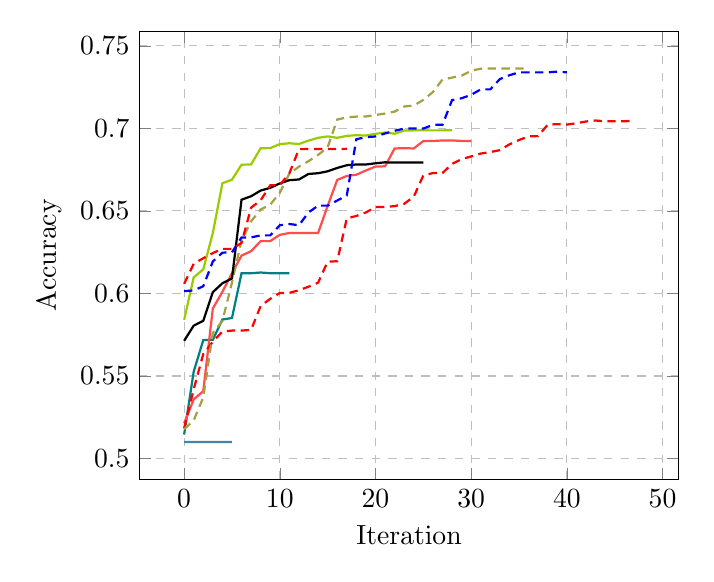
\begin{tikzpicture}
\begin{axis}[
    %title={Training},
    %width=0.8\textwidth,
    %height=0.5\textwidth,
    xlabel={Iteration},
    ylabel={Accuracy},
    %xmin=1, xmax=17,
    %ymin=0.44, ymax=1.1,
    %xtick={2,1024,2048,4096},
    %ytick={0.5,0.6,0.7,0.8,0.9,1.00},
    legend pos=south east,
    ymajorgrids=true,
    xmajorgrids=true,
    grid style=dashed,
    %xmode=log,
    %log ticks with fixed point,
    cycle list name = exotic,
    %cycle list = {
        %{black, mark=square, solid},
        %{red, mark=*, dotted},
        %{green, mark=x, dashed},
        %{blue, mark=+, dash dot},
        %{cyan, mark=o, dash dot dot},
        %{magenta, mark=asterisk, densely dotted},
        %{orange, mark=oplus, densely dashed},
        %{gray, mark=triangle, densely dash dot},
        %{lightgray, mark=diamnond, densely dash dot dot},
        %{brown, mark=star, loosely dotted},
    %}
]

%\begin{scope}[thick, mark options={scale=1.5, solid}]
\begin{scope}[thick, mark=none]
\addplot coordinates{
(0,0.51455)
(1,0.552633)
(2,0.571733)
(3,0.571933)
(4,0.584183)
(5,0.585117)
(6,0.612233)
(7,0.612233)
(8,0.612667)
(9,0.612233)
(10,0.612233)
(11,0.612233)
};
\addplot coordinates{
(0,0.509933)
(1,0.509933)
(2,0.509933)
(3,0.509933)
(4,0.509933)
(5,0.509933)
};
\addplot coordinates{
(0,0.509933)
(1,0.50995)
(2,0.509933)
(3,0.509933)
(4,0.509933)
(5,0.50995)
};
\addplot coordinates{
(0,0.521383)
(1,0.5358)
(2,0.5408)
(3,0.590883)
(4,0.601)
(5,0.612233)
(6,0.622933)
(7,0.625583)
(8,0.631683)
(9,0.631683)
(10,0.6355)
(11,0.6366)
(12,0.6366)
(13,0.6366)
(14,0.6366)
(15,0.653)
(16,0.668767)
(17,0.671133)
(18,0.671933)
(19,0.674483)
(20,0.676833)
(21,0.677017)
(22,0.687817)
(23,0.688)
(24,0.687817)
(25,0.692333)
(26,0.692333)
(27,0.692667)
(28,0.692667)
(29,0.692383)
(30,0.692333)
};
\addplot coordinates{
(0,0.583983)
(1,0.609767)
(2,0.61455)
(3,0.636583)
(4,0.666767)
(5,0.668883)
(6,0.677983)
(7,0.678117)
(8,0.688)
(9,0.688017)
(10,0.690467)
(11,0.690967)
(12,0.690533)
(13,0.692583)
(14,0.694267)
(15,0.695133)
(16,0.694283)
(17,0.695433)
(18,0.695867)
(19,0.69565)
(20,0.696683)
(21,0.697483)
(22,0.69675)
(23,0.698683)
(24,0.698767)
(25,0.6988)
(26,0.698767)
(27,0.698767)
(28,0.698867)
};
\addplot coordinates{
(0,0.5183)
(1,0.541933)
(2,0.5633)
(3,0.57075)
(4,0.576933)
(5,0.577483)
(6,0.577483)
(7,0.57795)
(8,0.592433)
(9,0.596733)
(10,0.600233)
(11,0.600367)
(12,0.601933)
(13,0.6041)
(14,0.6065)
(15,0.619283)
(16,0.619483)
(17,0.64545)
(18,0.64695)
(19,0.649067)
(20,0.652267)
(21,0.652383)
(22,0.652883)
(23,0.654283)
(24,0.6586)
(25,0.671467)
(26,0.672917)
(27,0.672933)
(28,0.678433)
(29,0.68135)
(30,0.683)
(31,0.684717)
(32,0.685667)
(33,0.686783)
(34,0.6903)
(35,0.69295)
(36,0.69515)
(37,0.695317)
(38,0.702233)
(39,0.70255)
(40,0.7023)
(41,0.703067)
(42,0.704167)
(43,0.70475)
(44,0.70425)
(45,0.704267)
(46,0.70425)
(47,0.704633)
};
\addplot coordinates{
(0,0.517783)
(1,0.52315)
(2,0.53705)
(3,0.576033)
(4,0.58325)
(5,0.606567)
(6,0.63205)
(7,0.643667)
(8,0.650867)
(9,0.653783)
(10,0.660933)
(11,0.67255)
(12,0.676783)
(13,0.680133)
(14,0.6839)
(15,0.688467)
(16,0.70535)
(17,0.706617)
(18,0.707117)
(19,0.707167)
(20,0.7081)
(21,0.708967)
(22,0.71015)
(23,0.713233)
(24,0.713783)
(25,0.717233)
(26,0.722)
(27,0.729567)
(28,0.730733)
(29,0.731917)
(30,0.7349)
(31,0.736133)
(32,0.73625)
(33,0.73625)
(34,0.73625)
(35,0.73625)
(36,0.736133)
};
\addplot coordinates{
(0,0.571317)
(1,0.580483)
(2,0.5834)
(3,0.60075)
(4,0.60615)
(5,0.609067)
(6,0.656783)
(7,0.658883)
(8,0.662333)
(9,0.66395)
(10,0.66665)
(11,0.6686)
(12,0.669033)
(13,0.672383)
(14,0.672817)
(15,0.673983)
(16,0.676017)
(17,0.677667)
(18,0.6781)
(19,0.6781)
(20,0.678833)
(21,0.679417)
(22,0.679267)
(23,0.679267)
(24,0.679267)
(25,0.679267)
};
\addplot coordinates{
(0,0.601417)
(1,0.6018)
(2,0.60435)
(3,0.619367)
(4,0.624683)
(5,0.6249)
(6,0.633917)
(7,0.633933)
(8,0.635167)
(9,0.635167)
(10,0.6413)
(11,0.64205)
(12,0.6413)
(13,0.64905)
(14,0.653183)
(15,0.653183)
(16,0.656283)
(17,0.65935)
(18,0.6934)
(19,0.694683)
(20,0.695067)
(21,0.696917)
(22,0.698533)
(23,0.69985)
(24,0.699867)
(25,0.699883)
(26,0.702117)
(27,0.70215)
(28,0.717083)
(29,0.718233)
(30,0.7203)
(31,0.723617)
(32,0.723617)
(33,0.72985)
(34,0.732183)
(35,0.7339)
(36,0.733917)
(37,0.733917)
(38,0.733917)
(39,0.734367)
(40,0.733917)
};
\addplot coordinates{
(0,0.605817)
(1,0.617967)
(2,0.6213)
(3,0.62445)
(4,0.626983)
(5,0.626983)
(6,0.6306)
(7,0.65195)
(8,0.656433)
(9,0.6655)
(10,0.665667)
(11,0.672783)
(12,0.6874)
(13,0.68745)
(14,0.687433)
(15,0.687433)
(16,0.687433)
(17,0.6876)
};
\end{scope}

\end{axis}
\end{tikzpicture}
\end{document}
